\documentclass[11pt,a4paper]{scrartcl}
\typearea{12}
\usepackage{graphicx}
\usepackage{pstricks}
\usepackage{listings}

\usepackage{tikz}

\usepackage{pgf}
\usepackage[utf8]{inputenc}
\usetikzlibrary{arrows,automata}
\usetikzlibrary{positioning}


\tikzset{
    neuron/.style={
           rectangle,
           rounded corners,
           draw=black, very thick,
           inner sep=2pt,
           text centered,
           },
}



\tikzset{
    area/.style={
           rectangle,
           draw=black, very thick,
           inner sep=2pt,
           text centered,
           },
}


\tikzset{
    gc/.style={
           rectangle,
           rounded corners,
           draw=red, very thick,
           inner sep=2pt,
           text centered,
           },
}


\tikzset{
    inh/.style={
           rectangle,
           rounded corners,
           draw=blue, very thick,
           inner sep=2pt,
           text centered,
           },
}



\tikzset{
    io/.style={
           rectangle,
           draw=green, very thick,
           inner sep=2pt,
           text centered,
           },
}



\lstset{language=python}
\pagestyle{headings}
\markright{Computational Neuroscience - 12 cerebellum}
\begin{document}

\subsection*{Introduction}
These notes are about the cerebellum and is partly based on \cite{Albus1971a}.

\subsection*{Anatomy of the cerebellum}
The cerebellum has a number of striking features; it has a more
stereotypical structure than most brain area and this structure is
conaerved across species. It also has one of the brain's largest cells,
the Purkinje cell, and its most numerous, the granule cell.

\begin{figure}
\begin{center}
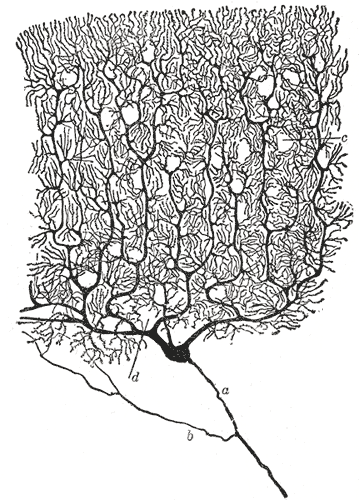
\includegraphics[width=7cm]{Purkinje_cell_by_Cajal.png}
\end{center}
\caption{A drawing by Santiago Ram\'{o}n y Cajal of a Purkinje cell. [Picture taken from \texttt{http://en.wikipedia.org/wiki/Golgi's\_method}]\label{fig:PC}}
\end{figure}

Purkinje cells have a distinctive structure with a huge, highly
branched, but flat dendritic arbor, see Fig.~\ref{fig:PC}; this allows
an extensive connectivity with each Purkinje cell receiving inputs
from around 100,000 other cells. In the cerebellum the Purkinje cell
are lined up like pages in a book, with their arbors lying in parallel
planes. They receive two excitatory inputs, weak inputs from parallel
fibres, axons that run perpendicular to the planes of the Purkinje
cell dendritic arbors, and a strong input from a climbing fibre, a
single axon which winds around the Purkinje cell and makes multiple
contacts with it, see Fig.~\ref{fig:cerebellum}.

\begin{figure}
\begin{center}
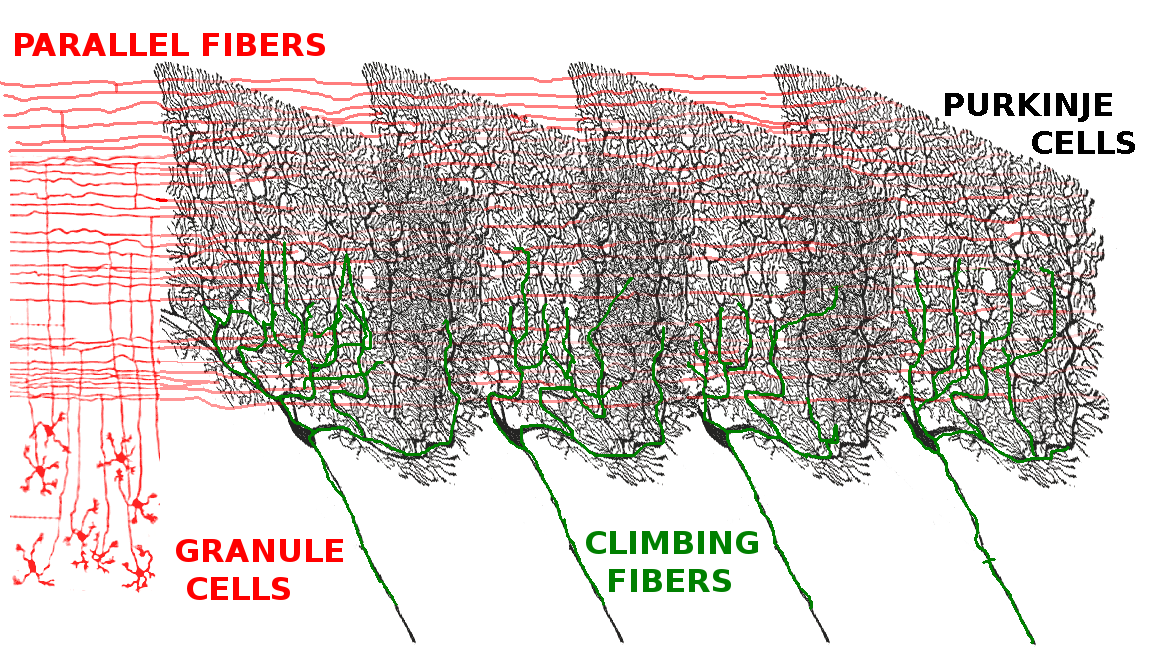
\includegraphics[width=11cm]{cerebellum.png}
\end{center}
\caption{A cartoon of the cerebellar circuitary. A vertical axon rises
  from each granule cells, splits once and then extends horizontally
  in two directions making connections with multiple Purkinje
  cells. Each Purkinje cell has its own climbing fiber which winds up
  around it.\label{fig:cerebellum}}
\end{figure}


\begin{figure}
\begin{center}
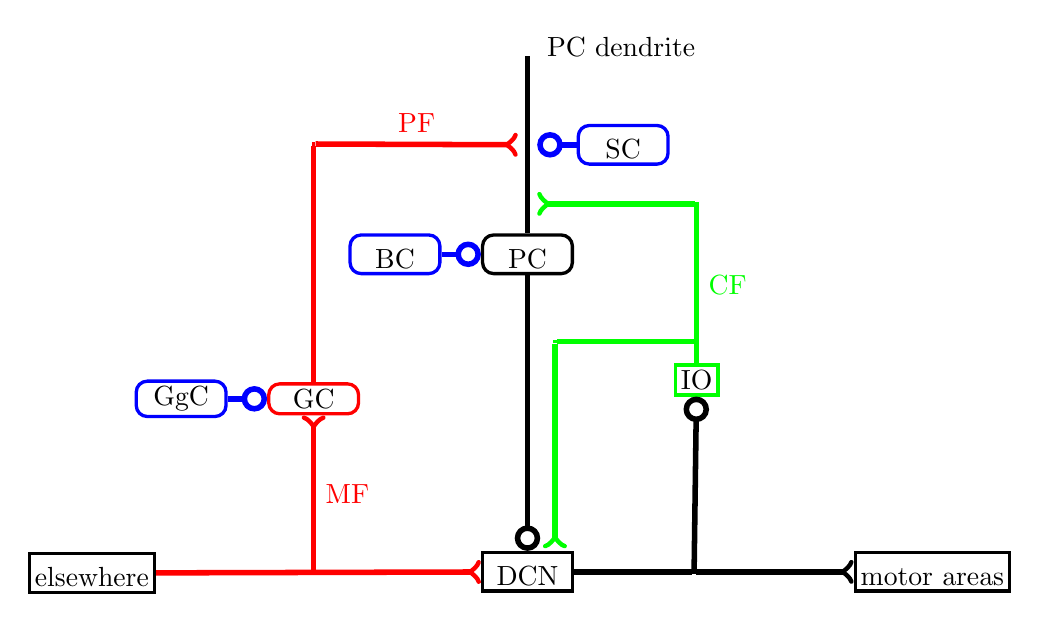
\begin{tikzpicture}
\node[neuron,text width=1cm, text height=0.35cm](PC){PC};
\node[inh,text width=1cm, text height=0.35cm,left = 0.5cm of PC](BC){BC};
\node[above = 1cm of PC](PCd){};
\node[inh,text width=1cm, text height=0.35cm,right = 0.5cm of PCd](SC){SC};
\node[above = 0.25cm of PC](PCc){};
\node[scale = 0.2,fill=green,right = 2cm of PCc](PCcr){};
\node[above = 1cm of PCd](PCdd){};
\node[right = 0cm of PCdd](){PC dendrite};
\node[left = 2cm of PC](PCl){};
\node[gc,text width=1cm,below = 1.5cm of PCl](GC){GC};
\node[inh,text width=1cm,left = 0.5cm of GC](GgC){GgC};
\node[scale = 0.2,fill=red,above = 3cm of GC](GCa){};
\node[scale = 0.01,fill=red,below = 2cm of GC](GCb){};
\node[io,below = 2cm of PCcr](IO){IO};
\node[scale =0.2,fill=green,above = 0.25cm of IO](IOa){};
\node[scale =0.2,fill=green,left = 1.75cm of IOa](IOl){};
\node[scale =0.01,below = 2.6cm of IOl](IOlb){};
\node[area,text width=1cm, text height=0.35cm,below  = 3.5cm of PC](DCN){DCN};
\node[scale=0.2,fill=black,right= 1.5cm of DCN](DCNr){};
\node[area,text height=0.35cm,right = 2cm of DCNr](ma){motor areas};
\node[area,text height=0.35cm,left = 2cm of GCb](ew){elsewhere};
\path (PCdd) edge[-,line width=2pt](PC);
\path (PC) edge[-o,line width=2pt] (DCN);
\path (IO) edge[-,green,line width=2pt] node[anchor=west]{CF} (PCcr);
\path (PCcr) edge[-<,green,line width=2pt] (PCc);
\path (GC) edge[-,red,line width=2pt] (GCa);
\path (GCa) edge[-<,red,line width=2pt] node[anchor=south]{PF}(PCd);
\path (GCb) edge[-<,red,line width=2pt] node[anchor=west]{MF} (GC);
\path (ew) edge[-<,red,line width=2pt] (DCN);
\path (DCN) edge[-,black,line width=2pt] (DCNr);
\path (DCNr) edge[-o,black,line width=2pt] (IO);
\path (DCNr) edge[-<,black,line width=2pt] (ma);
\path (IOa) edge[-,green,line width=2pt](IOl);
\path (IOl) edge[-<,green, line width=2pt](IOlb);
\path (GgC) edge[-o,blue, line width=2pt](GC);
\path (BC) edge[-o,blue, line width=2pt](PC);
\path (SC) edge[-o,blue, line width=2pt](PCd);
\end{tikzpicture}
\end{center}
\caption{A schematic of the cerebellar circuit. The granule cells (GC)
  receive input from a diverse range of other parts of the brain along
  the mossy fibers (MF). Each granule cell will combine input from
  just three or four mossy fibers and do this in lots of different
  combinations. The parallel fiber (PF) carries spikes from the GC to
  the Purkinje cell (PC) whose large dendrite is drawn as a line. The
  PC also receives input from a climbing fiber (CF) coming from
  Inferior Olivary Nucleus (IO). In turn it sends an inhibitory signal
  to the Deep Cerebellar Nucleus (DCN); the DCN has inhibitory neurons
  which act on IO and excitatory neurons which act on the motor
  system. The basket cells (BC), the Golgi cells (GgC) and the
  stellate cells (SC) are all local inhibitory
  cells.\label{fig:connectivity}}
\end{figure}

Another peculiarity is that the Purkinje cell has different responses
to different inputs; in response to multiple weak inputs from the
parallel fibers it fires a normal sort of spike, called in this
context a \textsl{simple spike}; in response to single spike from the
climbing fiber is fires a special spike, called a \textsl{complex
  spike}, with a leading spike, a number of small \lq{}spikelets\rq{}
and a sustained after-period of depolarization; this is illustrated in
Fig.~\ref{fig:spikes}.

\begin{figure}
\begin{center}
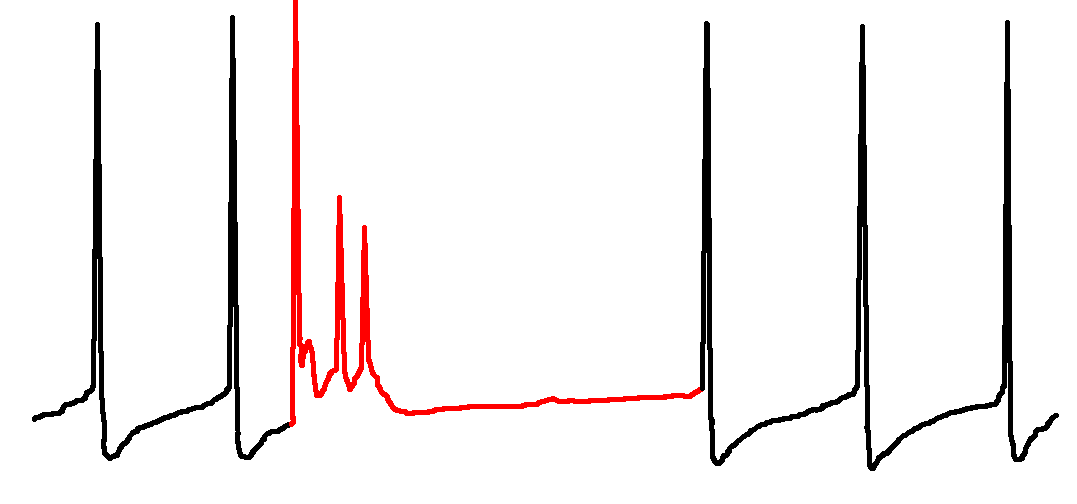
\includegraphics[width=8.cm]{complex_spike.png}
\end{center}
\caption{A complex spike. This drawing shows a simple spikes in black
  and a complex spike in red. The complex spike is followed by a long
  refractory period during which spiking is not possible. This is a
  sketch, not an actual recording, but a typical time scale would have
  this refractory period 50 ms long.\label{fig:spikes}}
\end{figure}

\subsection*{The Marr-Albus model}

It is still unclear exactly what the cerebellum does; what is known is
that it is important for actions, fine motor control and
proprioception; problems with the cerebellum are associated with
ataxia, loss of fine motor control, poor motor learning and poor
balance. There is a specific gait associated with cerebellar damage,
one that exhibits a certain self-consciousness or vigilance is
required for movement. According to most ideas about cerebellar
function it is required for the calculation of fine motor signals
\cite{Albus1971a}, or for predicting the sensory or proprioceptive
consequences of motor actions \cite{GaoEtAl1996a}.

Whatever exactly it does, it is widely believed, in accordance with
the Marr-Albus model \cite{Marr1969a,Albus1971a}, that the connections
from parallel fibers to Purkinje cells acts as a perceptron. Thus, if
$y$ is the output of the Purkinje cell and, in this simple model,
taking into account the fact Purkinje cells are inhibitory
\begin{equation}
y=-\sum{w_ix_i}
\end{equation}
where the $x_i$s are the activities in the parallel fibers and $w_i$
is the strength of the synapse from the $i$th parallel fiber to the
Purkinje cell. According to the perceptron rule there is a desired output $d$ and the synapses are adjusted according to
\begin{equation}
\Delta w_i=-\eta (d-y)x_i
\end{equation}
where $\eta$ is a small learning rate. The idea in the Marr-Albus
model is that the climbing fiber carries the error signal $d-y$.

Thus, in a simple example, say $\mathbf{w}=(1,1,1,1)$ initially and
the input $\mathbf{x}=(1,0,1,0)$ is supposed to have the output
$d=-1$, well
\begin{equation}
y=-\mathbf{w}\cdot\mathbf{x}=-2
\end{equation}
so $d-y=1$ and $\Delta\mathbf{w}=-\eta(1,0,1,0)$, so if $\eta=0.25$ after learning we would have $\mathbf{w}=(0.75,1,0.75,1)$ so
\begin{equation}
y=-\mathbf{w}\cdot\mathbf{x}=-1.5
\end{equation}
and the error has fallen to $d-y=0.5$. Conversely, imagine
$\mathbf{w}=(1,1,1,1)$ but $\mathbf{x}=(1,1,0,0)$ is intended to
represent $d=-3$, here
\begin{equation}
y=-\mathbf{w}\cdot\mathbf{x}=-2
\end{equation}
so $d-y=-1$ and $\Delta\mathbf{w}=-\eta(-1,-1,0,0)$ and after learning
with $\eta=0.25$ we would have $\mathbf{w}=(1.25,1.25,1,1)$. In other
words, we need both positive and negative errors with positive errors
associated with synaptic depression and negative errors with synaptic
potentiation; these have been observed experimentally
\cite{ItoEtAl1982a,DeanEtAl2010a} with climbing fibre activity greater
than or less than average corresponding to decreases and increases in
synapse strengths.

This can only be part of the description of this network. For example,
synapses form the parallel fibers can only be positive, not negative;
this can be accounted for by including inhibitory cells in the
network. Furthermore, a linear model like that being used here can't
learn complicated patterns like the XOR pattern:
\begin{center}
\begin{tabular}{llr}
$x_1$&$x_2$&$d$\\
\hline\\
0&0&0\\
0&1&-1\\
1&0&-1\\
1&1&0
\end{tabular}
\end{center}
Learning a pattern like this requires a network with more than one
layer; in fact, this is already provided by the granule cell
layer. Each granule cell receives input from between one and seven
mossy fibers, there are $3\times 10^{11}$ granule cells, roughly 100
to 150 times the number of mossy fibers. Finally there are large
inhibitory cells called Golgi cells in the network, these have long
time constants, providing delays; this is clearly useful for motor
control where different muscles move at different times or different
motor consequence unfold at different times during a motion
\cite{Fujita1982a,ShidaraEtAl1993a}.

This leaves lots of things mysterious; how this needs to be changed to
account for real spiking neurons, how the error signal adjusts the
synapse strengths, see \cite{Houghton2014a} for a suggest, and why
this very special architecture is ideal for this sort of
calculation. Another question relates to the error; our brain sees
muscles and nerves, our observation sees objects and motion, how are
the two reconciled: when you throw a dart you can see you hit the one
instead of the triple 20, you can't see which finger muscle was
activated too strongly or too weakly. However, with a low learning
rate $d$, or even $d-y$ isn't needed exactly, in fact, just the sign
is needed; that is something that could plausibly be deduced in
cortex.


\begin{thebibliography}{10}

\bibitem{Albus1971a}
Albus, JS. (1971) A theory of cerebellar function. 
\newblock Mathematical Biosciences 10: 25--61.

\bibitem{GaoEtAl1996a}
Gao J-H, Parsons LM, Bower JM, Xiong J, Li J and Fox PT (1996) Cerebellum implicated in sensory acquisition and discrimination rather than motor control.

\newblock Science 272: 545--7. 
\bibitem{Marr1969a}
Marr D (1969) A theory of cerebellar cortex.
\newblock Journal of Physiology 202: 437--70.

\bibitem{ItoEtAl1982a}
Ito M, Sakurai M and Tongroach P. (1982) Climbing fibre induced depression of both mossy fibre responsiveness and glutamate sensitivity of cerebellar Purkinje cells. 
\newblock Journal of Physiology, 324: 113--34.

\bibitem{DeanEtAl2010a}
Dean P, Porrill J, Ekerot CF and J\"{o}rntell H. (2010). The cerebellar microcircuit as an adaptive filter: experimental and computational evidence. 
\newblock Nature Reviews Neuroscience, 11: 30--43.

\bibitem{Fujita1982a}
Fujita M. (1982) Adaptive filter model of the cerebellum. 
\newblock Biological cybernetics, 45: 195--206.


\bibitem{ShidaraEtAl1993a}
Shidara M, Kawano K, Gomi H and Kawato M (1993) Inverse-dynamics model eye movement control by Purkinje cells in the cerebellum.
\newblock Nature, 365: 50--2.

\bibitem{Houghton2014a} Houghton C (2014) Supervised Learning with Complex Spikes and Spike-Timing-Dependent Plasticity. 
\newblock PLoS ONE 9(6): e99635. 

\end{thebibliography}

\end{document}
